\documentclass[10pt,a4paper]{article}
\usepackage[latin1]{inputenc}
\usepackage{amsmath}
\usepackage{amsfonts}
\usepackage{amssymb}
\usepackage{graphicx}
\usepackage[obeyspaces]{url}
\usepackage[colorlinks,urlcolor=blue]{hyperref}


\title{Windows installation guide for Abaqus 2016}
\date{} % blank date

% NOTE
% If you choose a folder for the abaqus working directory that isn't the default (C:\temp) and it doesn't yet exist, none of the shortcuts work.
% The start menu shortcuts will have nothing in the "start in" entry, but will work again if you create the folder and set this "start in" directory.
\begin{document}
	\maketitle
	\section{Licence Requirements}
	Before installing Abaqus please read the \href{https://www.applications.itservices.manchester.ac.uk/show_product.php?id=184&tab=licensing}{licence requirements}, in particular noting:
	
	Only appropriately authorised support staff may make physical copies of the software or documentation.
	Abaqus may only be installed on computers owned by the University of Manchester; it may not be installed on computers owned by staff or students.
	With limited exceptions use of Abaqus by students is limited to on-campus facilities.
	ABAQUS on-line documentation may not be made available over the open internet.
	
	
	\section{Supported compilers for Abaqus 2016}
	\subsection{C++ Compiler}
	Visual Studio 2012 Update 4 (available from ESD)
	
	\subsection{Fortran Compiler}
	Intel� Fortran Composer XE 2011 Update 6\\ \href{http://registrationcenter-download.intel.com/akdlm/irc_nas/2308/l_fcompxe_2011.6.233.tgz}{Download the installer}\\
	\href{https://www.applications.itservices.manchester.ac.uk/show_content_staffstud.php?id=142&pid=}{Installation guide}
		
	\section{Installation}
	There are 4 installers which have to be run in the following order:
	\begin{enumerate}
		\item Documentation
		
			Note that installing the documentation locally is optional. The alternative is to specify \url{http://50.16.225.63/v2016/} during the CAE installation.
		
		\item Services (solvers)
		\item CAA developer
		\item CAE
	\end{enumerate}

	It's generally just a process of double-clicking on each setup.exe in turn and accepting the defaults, but some details are given below for key steps. 
	
	\subsection{Documentation (optional)}
	\label{sec:documentation}
	Mount the iso file containing the documentation installer \path{Abaqus_fesafe_2016_documentation.iso}
	Run this installer\\ \path{\1\DOC_SIMULIA_Abaqus_fe-safe\1\Abaqus_2016\setup.exe}\\	
	Choose HTML and pdf
	
	\includegraphics[width=\textwidth]{"abaqus2016_documentation".PNG}
	
	\vspace{3mm}
	
	Make a note of the link provided at the end of the installation which is required to view the documentation in a web browser (shown in the red box below). You are required to enter this later on in the installation process.
	
	\vspace{3mm}
		
	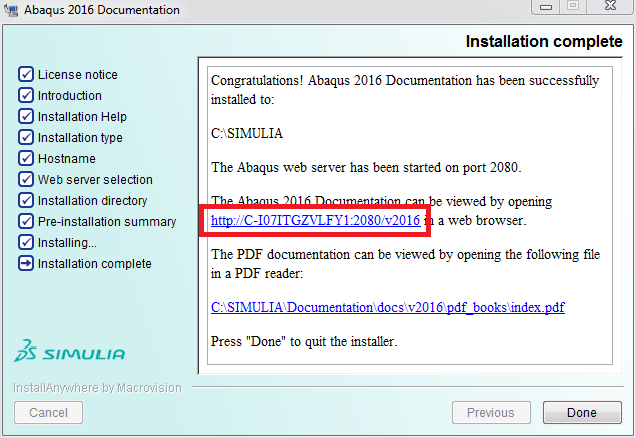
\includegraphics[width=\textwidth]{abaqus2016_documentation_complete_redbox}
	
	
	\subsection{Services (solvers)}
	Mount the iso file containing the Abaqus installers \path{Abaqus_2016_Win_Lin.iso}. This will show up as \path{Abaqus2016}.
	Run the installer
	% Full paths for downloaded media are longer - I only archived the relevant folders for ESD,
	% removing the leading "AM_SIM_Abaqus_Extend.AllOS\1"
	%\AM_SIM_Abaqus_Extend.AllOS\1\3DEXPERIENCE_AbaqusSolver\Windows64\1\setup.exe
	
	\path{Abaqus2016\3DEXPERIENCE_AbaqusSolver\Windows64\1\setup.exe}
	
	\subsection{CAA developer}
	Run the installer
	\path{Abaqus2016\CAA_3DEXPERIENCE_AbaqusSolver\Windows64\1\setup.exe}
	
	\subsection{CAE}
	Run the installer
	\path{Abaqus2016\SIMULIA_Abaqus_CAE\Windows64\1\setup.exe}
	
	Choose Flexnet as the licence type and enter the licence server:\\
	\texttt{28003@lfarm4.its.manchester.ac.uk}
	 
	There is a known bug in this version of Abaqus which causes the installation to fail if you enter the two redundant licence servers (\texttt{28003@lfarm5.its.manchester.ac.uk} and \texttt{28003@lfarm6.its.manchester.ac.uk})- this should be fixed in following releases.
	
	\vspace{3mm}
	
	\includegraphics[width=\textwidth]{"abaqus2016_licence_details_known_bug".png}
	
	\vspace{3mm}
	
	When prompted to enter a location for the documentation, either enter \url{http://50.16.225.63/v2016/} or the location you made a note of in section \ref{sec:documentation}.
	
	\subsubsection{A warning about the working directory}
	You will be asked to choose a location for the Abaqus working directory. By default, this is \path{C:\temp} and this will be created if it doesn't already exist. If you want to use a different directory, make sure it exists. The text box suggests you can specify a path to be created (by changing the default \path{C:\temp}), however the installer won't create a new directory for you, and Abaqus won't install properly.
	
	\subsubsection{Subset verification suite}
	As part of the installation process, Abaqus will run the verification suite and report the results. Note this is only a sub-set of the verification suite, so the verification should be run again post-installation.
	
	\section{Post-installation tasks}
	\subsection{Modify shortcuts to get user subroutines working}
	To get User Subroutines working with Intel Compiler XE 2011, copy \\ \path{Abaqus2016\abaqus_set_env.bat} to \path{C:\SIMULIA\} and then modify the Abaqus start menu shortcuts thus:
	\begin{enumerate}
		\item Go to the \textbf{Start Menu $\rightarrow$ All Programs $\rightarrow$ Dassault Systemes SIMULIA Abaqus CAE 2016}, right click on \textbf{Abaqus CAE}, then left click on \textbf{properties}
		\item Copy and paste the below string (everything within, but not including the quote marks) to the very beginning of the \textbf{Target} field. Ensure there is a single space either side of the final ``\textbf{\&\&}''\\
		\path{"C:SIMULIA\abaqus_set_env.bat && "}
		\item Repeat this for the Abaqus Command and Abaqus Verification shortcuts in the \textbf{Dassault Systemes SIMULIA Abaqus CAE 2016} sub-menu
	\end{enumerate}
	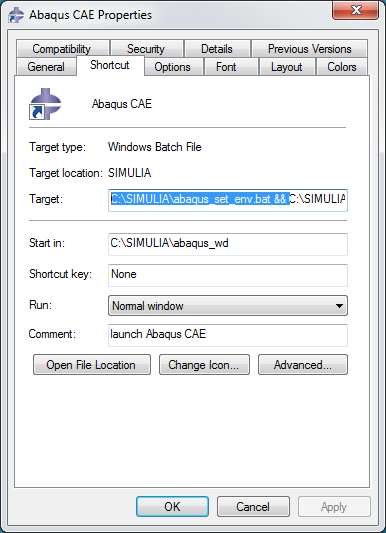
\includegraphics{abaqus2016_start_menu_modification}
	
	\subsection{Verification suite}
	Run the verification suite to test the installation was successful. Start Menu $\rightarrow$ All Programs $\rightarrow$ Dassault Systemes SIMULIA Abaqus CAE 2016 $\rightarrow$ Abaqus verification. Tests should report PASS (or skipped for unlicensed features) in the verify.log file. If Abaqus has not been configured correctly to use the Fortran and C++ compilers then tests will fail for user subroutines and make utilities.
	
	
	
\end{document}
